\documentclass[border=2mm,12pt]{standalone}
\usepackage{tikz}

\begin{document}
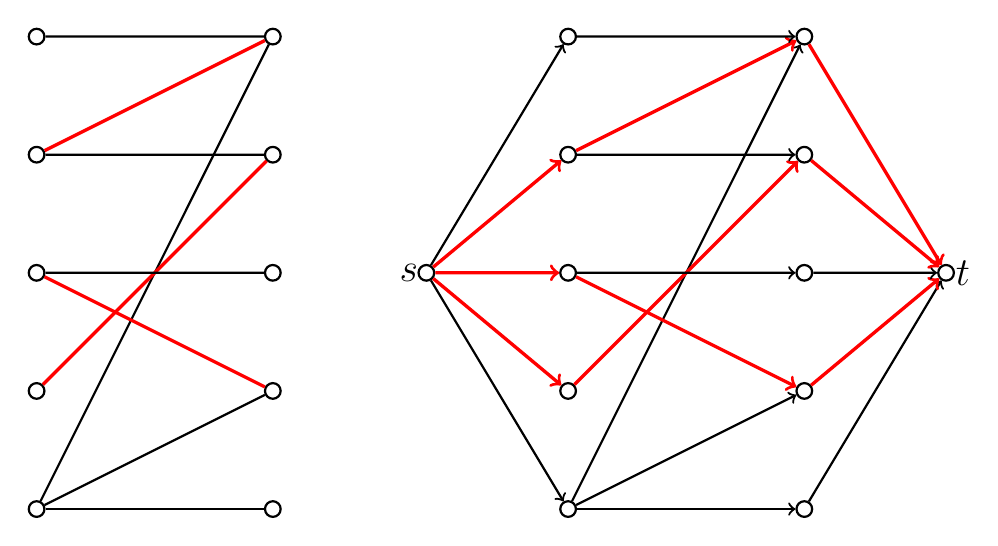
\begin{tikzpicture}[
    xscale=3, yscale=1.5, thick,
    every node/.style={draw, circle, inner sep=-2pt},
]

    \begin{scope}
    
        \node (x1) at (0,0) {};
        \node (x2) at (0,1) {};
        \node (x3) at (0,2) {};
        \node (x4) at (0,3) {};
        \node (x5) at (0,4) {};
        \node (y1) at (1,0) {};
        \node (y2) at (1,1) {};
        \node (y3) at (1,2) {};
        \node (y4) at (1,3) {};
        \node (y5) at (1,4) {};

        \draw (x1) -- (y1);
        \draw (x1) -- (y2);
        \draw (x1) -- (y5);
        \draw (x2) -- (y4) [very thick,red];
        \draw (x3) -- (y2) [very thick,red];
        \draw (x3) -- (y3);
        \draw (x4) -- (y4);
        \draw (x4) -- (y5) [very thick,red];
        \draw (x5) -- (y5);

    \end{scope}

    \begin{scope}[xshift=2.25cm]
    
        \node (x1) at (0,0) {};
        \node (x2) at (0,1) {};
        \node (x3) at (0,2) {};
        \node (x4) at (0,3) {};
        \node (x5) at (0,4) {};
        \node (y1) at (1,0) {};
        \node (y2) at (1,1) {};
        \node (y3) at (1,2) {};
        \node (y4) at (1,3) {};
        \node (y5) at (1,4) {};
        \node [label={[shift={(-1pt,0pt)}]left:\Large $s$}]  (s)  at (-0.6,2) {};
        \node [label=right:\Large $t$] (t)  at (1.6,2)  {};

        \draw[->] (x1) -- (y1);
        \draw[->] (x1) -- (y2);
        \draw[->] (x1) -- (y5);
        \draw[->] (x2) -- (y4) [very thick,red];
        \draw[->] (x3) -- (y2) [very thick,red];
        \draw[->] (x3) -- (y3);
        \draw[->] (x4) -- (y4);
        \draw[->] (x4) -- (y5) [very thick,red];
        \draw[->] (x5) -- (y5);

        \draw[->] (s)  -- (x1);
        \draw[->] (s)  -- (x2) [very thick,red];
        \draw[->] (s)  -- (x3) [very thick,red];
        \draw[->] (s)  -- (x4) [very thick,red];
        \draw[->] (s)  -- (x5);

        \draw[->] (y1) -- (t);
        \draw[->] (y2) -- (t) [very thick,red];
        \draw[->] (y3) -- (t);
        \draw[->] (y4) -- (t) [very thick,red];
        \draw[->] (y5) -- (t) [very thick,red];

    \end{scope}

\end{tikzpicture}
\end{document}
